\newpage
{\bfseries МРНТИ 20.15.05}
\hfill {\bfseries \href{https://doi.org/10.58805/kazutb.v.2.23-467}{https://doi.org/10.58805/kazutb.v.2.23-467}}

\sectionwithauthors{Ж. Бидахмет, Г.З. Зиятбекова, С.К. Заманова, Ж.Ж. Кожамкулова, А.К. Адильбекова, С.М. Жаксыбай}{АНАЛИЗ РАСШИРЕННЫХ ВОЗМОЖНОСТЕЙ СИСТЕМЫ SIEM ЧЕРЕЗ ИНТЕГРАЦИЮ С IBM QRADAR}

\begin{center}
{\bfseries \textsuperscript{1}Ж. Бидахмет, \textsuperscript{1}Г.З.
Зиятбекова\envelope, \textsuperscript{1}С.К. Заманова, \textsuperscript{2}Ж.Ж.
Кожамкулова, \textsuperscript{3}А.К. Адильбекова, \textsuperscript{1}С.М.
Жаксыбай}

\textsuperscript{2}Казахский национальный университет имени аль-Фараби,
Алматы, Казахстан,

\textsuperscript{2}НАО АУЭС имени Г. Даукеева, Алматы, Казахстан,

\textsuperscript{3}Казахский университет международных отношений и
мировых языков

имени Абылай хана, Алматы, Казахстан,

е-mail: zhaksybaysanzhar@gmail.com
\end{center}

В данной статье рассматриваются важные аспекты SIEM-технологии, роли в
кибербезопасности и ее компонентов, обсуждаются ключевая роль
SIEM-системы в современном мире информационных технологий, а также
рассмотрены основные компоненты SIEM-системы, включая сборщики данных,
системы корреляции, дэшборды и отчеты. Представлен код, являющийся
частью разработки, предназначенной для мониторинга сетевого трафика и
обнаружения потенциальных угроз, таких как DDoS-атаки. Основные
использованные технологии и методы описаны ниже.

{\bfseries Ключевые слова:} SIEM, IBM QRadar, DDoS-атака, информационная
безопасность, кибербезопасность, мониторинг, угроза.

\begin{center}
{\large\bfseries IBM QRADAR ИНТЕГРАЦИЯСЫ АРҚЫЛЫ SIEM ЖҮЙЕСІНІҢ КЕҢЕЙТІЛГЕН
МҮМКІНДІКТЕРІН ТАЛДАУ}

{\bfseries \textsuperscript{1}Ж. Бидахмет, \textsuperscript{1}Г.З.
Зиятбекова\envelope, \textsuperscript{1}С.К. Заманова, \textsuperscript{2}Ж.Ж.
Кожамкулова, \textsuperscript{3}А.К. Адильбекова, \textsuperscript{1}С.М.
Жаксыбай}

\textsuperscript{1}әл-Фараби атындағы Қазақ ұлттық университеті, Алматы,
Қазақстан,

\textsuperscript{2}Г. Даукеев атындағы КЕАҚ АЭжБУ, Алматы, Қазақстан,

\textsuperscript{3}Абылай хан атындағы ҚазХҚжӘТУ, Алматы, Қазақстан,

е-mail: zhaksybaysanzhar@gmail.com
\end{center}

Бұл мақалада SIEM технологиясының маңызды аспектілері, оның
киберқауіпсіздіктегі рөлі мен құрамдас бөліктері қарастырылады,
ақпараттық технологиялардың заманауи әлеміндегі SIEM жүйесінің негізгі
маңыздылығы талқыланады, сонымен қатар, SIEM жүйесінің негізгі құрамдас
бөліктері, соның ішінде дерек жинаушылар, корреляциялық жүйелер, бақылау
тақталары және есептер қарастырылады. Ұсынылған код желілік трафикті
бақылауға және DDoS шабуылдары сияқты ықтимал қауіптерді анықтауға
арналған әзірлеменің бөлігі болып табылады. Қолданылатын негізгі
технологиялар мен әдістер төменде сипатталған.

{\bfseries Түйін сөздер:} SIEM, IBM QRadar, DDoS шабуылы, ақпараттық
қауіпсіздік, киберқауіпсіздік, мониторинг, қауіп.

\begin{center}
{\large\bfseries ANALYZE SIEM SYSTEM ADVANCED FEATURES THROUGH INTEGRATION WITH
IBM QRADAR}

{\bfseries \textsuperscript{1}Zh. Bydakhmet, \textsuperscript{1}G.Z.
Ziyatbekova\envelope, \textsuperscript{1}S.K. Zamanova, \textsuperscript{2}Zh.Zh.
Kozhamkulova, \textsuperscript{3}A.K. Adilbekova, \textsuperscript{1}S.M.
Zhaksybay}

\textsuperscript{1}Al-Farabi Kazakh National University, Almaty,
Kazakhstan,

\textsuperscript{2}Non-profit joint-stock company {\bfseries ``}Almaty
University of Power Engineering and Telecommunications after Gumarbek
Daukeev'' Almaty, Kazakhstan,

\textsuperscript{3}Kazakh Ablaikhan university of international
relations and world languages,

Almaty, Kazakhstan,

е-mail: zhaksybaysanzhar@gmail.com
\end{center}

This article discusses important aspects of SIEM technology, the role in
cybersecurity and its components, discusses the key role of the SIEM
system in the modern world of information technology, and examines the
main components of the SIEM system, including data collectors,
correlation systems, dashboards and reports. The code is presented,
which is part of a development designed to monitor network traffic and
detect potential threats such as DDoS attacks. The main technologies and
methods used are described below.

{\bfseries Keywords:} SIEM, IBM QRadar, DDoS attack, information security,
cybersecurity, monitoring, threat.

\begin{multicols}{2}
{\bfseries Введение.} Системы управления информацией и событиями
безопасности (SIEM -- Security information and event management) начали
свое развитие в конце 1990-х -- начале 2000-х годов из простых систем
лог-менеджмента. Эти системы первоначально были созданы для сбора,
агрегирования и хранения лог-файлов от различных систем и устройств в
централизованном хранилище. Основной целью было обеспечить удобный
доступ к логам для целей аудита и устранения неисправностей. Со временем
возникла потребность в более продвинутом анализе данных для обнаружения
и предотвращения инцидентов безопасности.

\emph{Развитие функциональности: Корреляция и аналитика.} Как
развивались технологии и увеличивалось количество киберугроз, стало
очевидно, что простого сбора и хранения логов недостаточно. В ответ на
это появились системы, способные не только собирать данные, но и
анализировать их на предмет аномалий и угроз. Так родились первые
SIEM-системы, которые начали использовать правила для корреляции событий
и алертов, позволяя IT-специалистам и аналитикам безопасности более
эффективно реагировать на инциденты.

\emph{Внедрение технологий машинного обучения и больших данных}. С
развитием технологий больших данных и машинного обучения современные
SIEM-системы стали значительно мощнее. Они начали предлагать не только
реактивный, но и проактивный подход к безопасности. Это включало
поведенческий анализ и аналитику в реальном времени, что позволило
обнаруживать даже сложные угрозы, маскирующиеся под обыденную активность
в сети {[}1-2{]}.

\emph{Роль IBM QRadar в эволюции SIEM.} IBM QRadar является одним из
лидеров в области SIEM. Он был разработан для предоставления
комплексного решения по управлению сетевой безопасностью, которое
интегрирует сбор логов, мониторинг событий, их корреляцию и аналитику.
QRadar использует сложные алгоритмы для анализа и корреляции данных, что
позволяет обнаруживать угрозы более эффективно и в более ранние стадии,
чем традиционные системы. Эта эволюция отражает не только технический
прогресс, но и изменения в подходах к обеспечению безопасности, делая
современные SIEM-системы более адаптивными и интеллектуальными {[}3{]}.

\emph{Основные технологии и методы обнаружения угроз.} \emph{Примеры и
кейс-стади.} Примером сложной угрозы может служить атака через
беспроводные сети, где злоумышленники используют сетевые запросы для
распространения вредоносного ПО в пределах корпоративной сети. В таких
случаях SIEM системы, оснащенные инструментами для глубокого анализа
сетевого трафика и поведенческого мониторинга, могут быстрее обнаружить
и нейтрализовать угрозу.

Сложность и разнообразие современных киберугроз требуют от SIEM систем
не только быстрого реагирования, но и глубокого понимания контекста
каждой угрозы. Развитие технологий, таких как машинное обучение и
искусственный интеллект, помогает современным SIEM системам, включая IBM
QRadar, эффективно справляться с этими вызовами, предоставляя более
мощные и умные инструменты для защиты цифровых активов организаций
{[}4{]}.

\emph{Основные технологии.} \emph{Flask:} это легковесный веб-фреймворк
на языке Python, предназначенный для создания веб-приложений. В данном
контексте он используется для создания веб-интерфейса для мониторинга
сетевого трафика.

\emph{Scapy:} это мощная библиотека Python, которая позволяет
интерактивно работать с сетевыми пакетами. В коде используются модули
\emph{sniff, IP}, и \emph{TCP} из Scapy для перехвата и анализа сетевого
трафика.

\emph{Subprocess:} Модуль Python, используемый для запуска новых
приложений или программ, которые могут выполняться параллельно с
Python-скриптом.

\emph{Logging:} Модуль Python для логирования событий. В данном коде он
настраивается для сохранения записей о сетевом трафике в файл
\emph{network\_traffic.log}.

\emph{Nmap:} Инструмент для исследования сети и аудита безопасности.
Хотя он не показан в действии в представленном фрагменте кода, его можно
использовать для сканирования сети на наличие уязвимых портов {[}5-6{]}.

{\bfseries Материалы и методы.} \emph{Сбор данных:} Используя Scapy,
система перехватывает сетевой трафик и собирает данные о пакетах,
передаваемых через сеть.

\emph{Анализ портов:} В коде определены уязвимые порты
(\emph{vulnerable\_ports}), которые могут подвергаться сканированию или
атакам. Система может анализировать трафик на эти порты для обнаружения
подозрительной активности.

\emph{Обнаружение аномалий:} Установлен порог
(\emph{anomalous\_traffic\_threshold}) для обнаружения аномального
трафика. Если объем трафика превышает этот порог, система может
генерировать предупреждение о возможной аномалии.

\emph{DDoS обнаружение:} Порог (\emph{ddos\_threshold}) устанавливается
для обнаружения DDoS-атак. Это сделано для мониторинга необычно высокого
трафика, который может указывать на DDoS.

Использование этих технологий и методов в совокупности позволяет создать
систему, способную эффективно мониторить сетевой трафик и предупреждать
о потенциальных угрозах в реальном времени. Такая система становится
важной частью защитного механизма в контексте кибербезопасности,
дополняя возможности традиционных SIEM систем и повышая общую
защищенность сетевой инфраструктуры.

Практическое применение разработки: интеграция сетевого мониторинга и
анализа {[}7-8{]}.

{\bfseries Результаты и обсуждение.} \emph{Описание кода.} Код системы
(Рис. 1-4) начинается с импорта необходимых библиотек:
\end{multicols}

\begin{figure}[H]
	\centering
	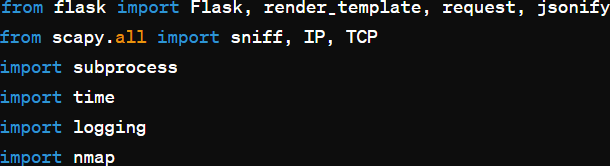
\includegraphics[width=0.7\textwidth]{assets/47}
	\caption*{Рис. 1 -- Импорт необходимых библиотек}
\end{figure}

Затем, настраивается базовая конфигурация логирования и создается
экземпляр Flask-приложения:

\begin{figure}[H]
	\centering
	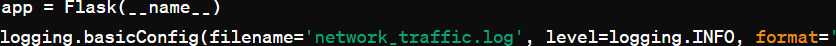
\includegraphics[width=0.9\textwidth]{assets/48}
	\caption*{Рис. 2 -- Flask-приложение}
\end{figure}

С помощью Scapy осуществляется захват пакетов и анализ сетевого трафика.
Каждый пакет обрабатывается функцией packet\_handler, которая извлекает
важные данные и хранит их в словаре:

\begin{figure}[H]
	\centering
	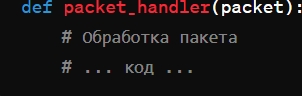
\includegraphics[width=0.4\textwidth]{assets/49}
	\caption*{Рис. 3 - Анализ сетевого трафика}
\end{figure}

В коде реализованы механизмы для определения аномального трафика и
обнаружения DDoS-атаки, а также функции для блокировки IP-адресов,
подозрительных в сканировании портов.

Примеры использования. Возьмем для примера функцию обнаружения
аномального трафика:

\begin{figure}[H]
	\centering
	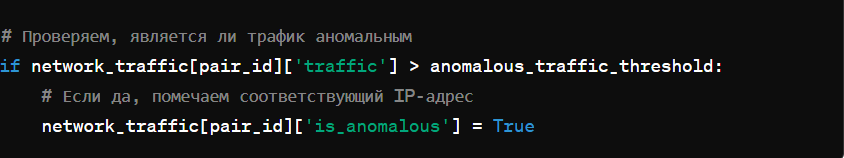
\includegraphics[width=0.9\textwidth]{assets/50}
	\caption*{Рис. 4 - Функция обнаружения аномального трафика}
\end{figure}

Этот фрагмент кода проверяет, превышает ли количество трафика для пары
IP-адресов установленный порог, и в случае обнаружения аномалии отмечает
соответствующий IP-адрес как аномальный.

Интеграция с Nmap для сканирования уязвимостей. Кроме того, мы
использовали

\emph{Цветовая индикация угроз.} Для улучшения восприятия информации и
скорости реагирования таблицы используют цветовую индикацию для
различных типов угроз (Рис. 5-7):

- Красный цвет выделяет уязвимые порты и потенциальные DDoS-атаки.

- Желтый цвет указывает на аномальный трафик.

- Зеленый цвет предупреждает о сканировании портов.

\begin{figure}[H]
	\centering
	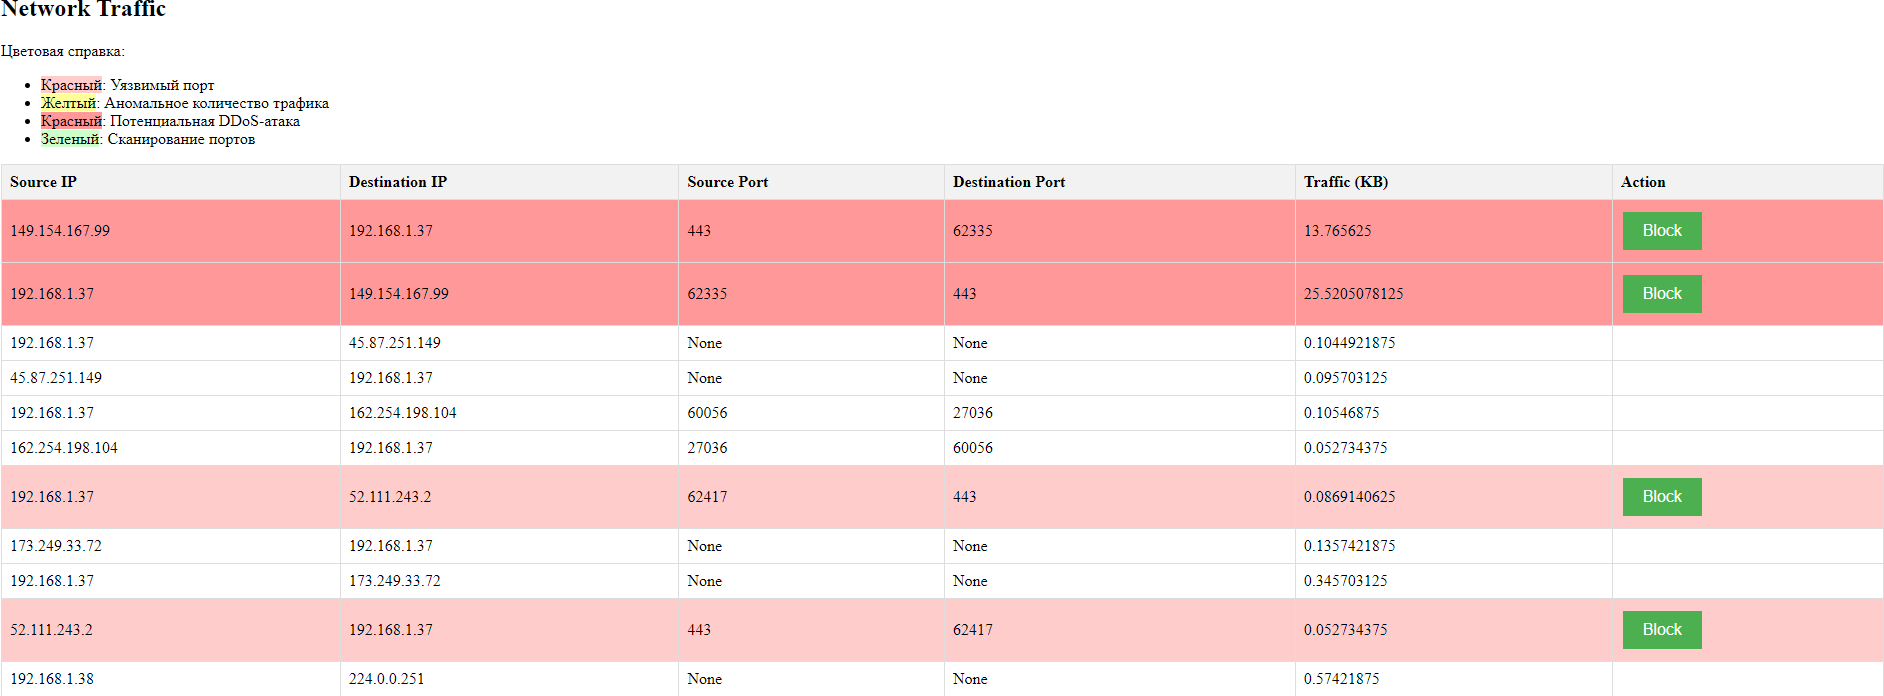
\includegraphics[width=0.8\textwidth]{assets/51}
	\caption*{Рис. 5 - Цветовая индикация угроз}
\end{figure}

\begin{figure}[H]
    \centering
    \begin{subfigure}[b]{0.45\textwidth}
        \centering
        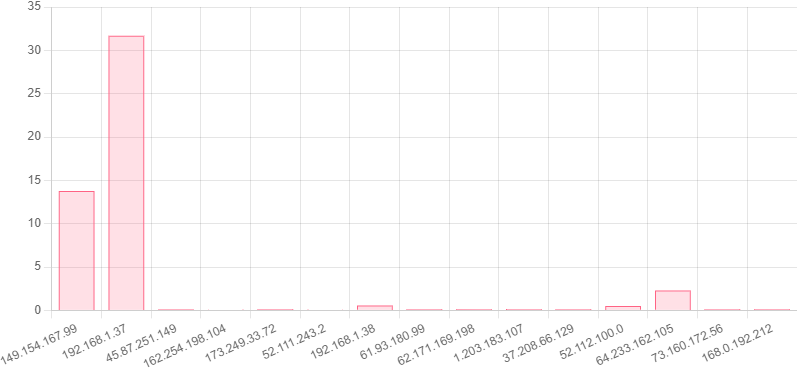
\includegraphics[width=\textwidth]{assets/52}
		\caption*{Рис. 6 - Исходящий трафик}
    \end{subfigure}
    \hfill
    \begin{subfigure}[b]{0.45\textwidth}
        \centering
        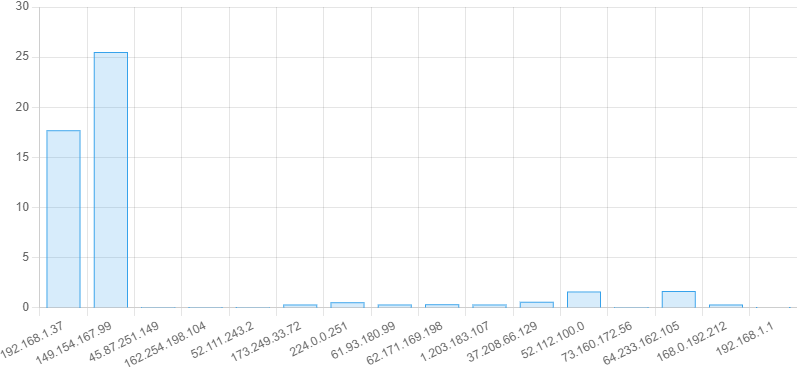
\includegraphics[width=\textwidth]{assets/52.1}
		\caption*{Рис. 7 - Входящий трафик}
    \end{subfigure}
\end{figure}

\begin{multicols}{2}
\emph{Обнаружение и предотвращение сканирования портов. Описание кейса:}
Средняя компания ABC, работающая в сфере финансовых услуг, столкнулась с
увеличением числа попыток несанкционированного сканирования портов в их
сети, что создавало потенциальные угрозы безопасности. Для защиты от
таких атак компания внедрила нашу систему мониторинга. Система
мониторинга непрерывно анализировала сетевой трафик и применяла
алгоритмы обнаружения сканирования портов для выявления подозрительной
активности. При обнаружении таких попыток система автоматически
блокировала исходящие запросы с подозрительных IP-адресов.

\emph{Эффективное обнаружение угроз:} Система успешно выявила и
предотвратила ряд попыток сканирования портов, минимизируя риски
нарушения безопасности и сокращая время необходимое для реагирования на
инциденты.

\emph{Повышение защищенности сети:} благодаря реакции в реальном времени
на угрозы, компания смогла улучшить общий уровень безопасности своей
сети и защитить конфиденциальные данные клиентов.

\emph{Сокращение операционных затрат:} Уменьшение количества атак на
сеть привело к сокращению времени, затрачиваемого на расследование
инцидентов и восстановление сервисов.

Рассмотренные кейс-стади являются лишь двумя примерами успешного
применения системы мониторинга сетевого трафика, разработанной нами. Эти
кейсы подчеркивают значимость эффективного мониторинга и оперативного
реагирования на угрозы для обеспечения безопасности и надежности
корпоративных сетей.

\emph{Тенденции и прогнозы в области SIEM, исследование текущих
тенденций.} Системы управления информационной безопасностью (SIEM)
продолжают развиваться, приспосабливаясь к новым вызовам и угрозам в
области кибербезопасности. Некоторые текущие тенденции в этой области
включают:

\emph{Облачные решения:} Возрастающая потребность в масштабируемых и
гибких решениях подталкивает компании к переходу от локальных SIEM
систем к облачным платформам, что позволяет более эффективно управлять
растущим объемом данных.

\emph{Искусственный интеллект и машинное обучение:} Использование
алгоритмов машинного обучения и искусственного интеллекта становится все
более распространенным в SIEM системах для более точного обнаружения и
анализа угроз.

\emph{Расширенный анализ данных:} Компании все больше осознают ценность
данных о безопасности не только для реагирования на инциденты, но и для
принятия стратегических решений в области кибербезопасности.

\emph{Будущие инновации.} В будущем можно ожидать дальнейшего развития
SIEM систем в следующих направлениях:

\emph{Автоматизация и оркестрация:} Развитие автоматизированных
процессов обнаружения и реагирования на угрозы позволит компаниям
сократить время реагирования на инциденты и улучшить эффективность своих
кибербезопасных операций.

\emph{Усиление аналитики:} Внедрение более продвинутых методов аналитики
данных, таких как анализ поведения пользователей и контекстной
информации, позволит более точно выявлять потенциальные угрозы.

\emph{Интеграция с другими технологиями:} SIEM системы будут все более
интегрироваться с другими технологиями кибербезопасности, такими как EDR
(Endpoint Detection and Response) и SOAR (Security Orchestration,
Automation, and Response), для обеспечения более полного и
согласованного подхода к безопасности {[}9{]}.

\emph{Вклад разработки в будущее индустрии.} Разработка представляет
собой важный шаг в направлении инновационных решений в области SIEM.
Таким образом продукт может формировать будущее систем SIEM:

\emph{Расширенные алгоритмы обнаружения:} Система предлагает расширенные
алгоритмы обнаружения аномального трафика, DDoS-атак и сканирования
портов, что позволяет более точно выявлять угрозы и снижать ложные
срабатывания.

\emph{Интеграция с облачными технологиями:} Интеграция системы с
облачными технологиями позволяет клиентам быстрее и легче масштабировать
свои кибербезопасные операции в соответствии с их потребностями.

\emph{Повышение эффективности операций:} Продукт обеспечивает более
быструю реакцию на угрозы благодаря автоматизации и оптимизации
процессов обнаружения и реагирования, что в конечном итоге позволяет
нашим клиентам сэкономить время и ресурсы.

\emph{Снижение времени реагирования:} благодаря системе мониторинга,
корпорация смогла оперативно реагировать на DDoS-атаки, минимизируя
временные простои и потери до минимума.

\emph{Увеличение доступности сервисов:} Применение системы позволило
значительно увеличить доступность онлайн-сервисов корпорации, повысив
удовлетворенность клиентов.

\emph{Экономические выгоды:} Подсчет экономических потерь, связанных с
DDoS-атаками, показал существенное сокращение убытков после внедрения
системы мониторинга {[}10{]}.

\emph{Взгляд в будущее.} Исследование показывает, что будущее SIEM
система будет определяться инновациями в области облачных технологий,
искусственного интеллекта и автоматизации процессов. Разработка играет
ключевую роль в этом развитии, предлагая расширенные алгоритмы
обнаружения, интеграцию с облачными платформами и повышение
эффективности операций кибербезопасности.

{\bfseries Выводы.} В заключении отражается текущие тенденции в области
SIEM, но и указывает на будущее направление развития этой индустрии.
Можно сказать, что вклад способствует укреплению кибербезопасности и
защите информационных ресурсов как для корпоративных клиентов, так и для
конечных пользователей.

Разработка не только предлагает инновационные технологические
возможности, но и способствует укреплению общей безопасности
информационных систем, что делает ее ключевым игроком в будущем развитии
индустрии SIEM. В статье рассмотрена эволюция систем управления
информационной безопасностью (SIEM) от простых лог-систем до современных
аналитических платформ. Обсуждена роль системы IBM QRadar в индустрии и
выявлены текущие вызовы, с которыми сталкиваются SIEM системы, включая
объем данных, сложность угроз и недостатки текущих решений.
\end{multicols}

\begin{center}
{\bfseries Литература}
\end{center}

\begin{noparindent}
1.David R. Miller,~ Shon Harris,~ Allen Harper,~ Stephen VanDyke,~ Chris
Blask Security Information and Event Management (SIEM) Implementation//
Mcgraw-hill , 2010.- 464 P. ISBN 978-0-07-170108-2

2.Vitalii Varkentin, Kseniia Nikolskaia. Особенности создания наборов
данных для обучения систем обнаружения вторжений, основанных на методах
машинного обучения. Сборник материалов конференции. СПб.: Изд-во СПбГЭТУ
«ЛЭТИ», 2019.- Т.1.- С. 141-143.

3.Joseph Muniz, Gary McIntyre, and Nadhem AlFardan. Security Operations
Center: Building, Operating, and Maintaining Your SOC Paperback// Gisco
Press.- 448 p. ISBN 978-0134052014

4.Richard Bejtlich. The Practice of Network Security Monitoring:
Understanding Incident Detection and Response, 2013. -376 р. ISBN
101-59327-509-9

https://terrorgum.com/tfox/books/practiceofnetworksecuritymonitoring.pdf

5.Gerardus Blokdyk. Security Information and Event Management (SIEM) --
A Complete Guide// ~5STARCooks, 2020.- 320 p. ISBN10:0655914668, ISBN
13:978-0655914662

https://www.amazon.com/Security-Information-Event-Management-Complete/dp/0655914668

6.Gustavo González-Granadillo, Susana González-Zarzosa and Rodrigo Diaz.
Security Information and Event Management (SIEM): Analysis, Trends, and
Usage in Critical Infrastructures// Sensors, 2021.- Vol.21(14), 4759.
https://doi.org/10.3390/s21144759

7.Rahman Ali, Asmat Ali, Farkhund Iqbal, Mohammed Hussain and Farhan
Ullah. Deep Learning Methods for Malware and Intrusion Detection: A
Systematic Literature Review// Security and Communication Networks,
2022.- Vol.22.- 31 р. https://doi.org/10.1155/2022/2959222

8.Yanli Shao, Yang Lu, Dan Wei, Jinglong Fang, Feiwei Qin and Bin Chen.
Malicious Code Classification Method Based on Deep Residual Network and
Hybrid Attention Mechanism for Edge Security// Wireless Communications
and Mobile Computing,2022.- Vol.2022.- 19 p.

DOI https://doi.org/10.1155/2022/3301718

9.Смирнов А.И. Глобальная безопасность: инновационные методы анализа
конфликтов. -- М.: Знание, 2013. -- 278 с.

10.Жаксыбай С.М. Управление событиями информационной безопасности с
помощью SIEM-системы// Интелектуальные технологии на транспорте,2023.-№
S1 (спецвыпуск).- С. 66- 69. https://ivs.pgups.ru/events/mmis-2023
\end{noparindent}

\begin{center}
{\bfseries References}
\end{center}

\begin{noparindent}
1.David R. Miller,~ Shon Harris,~ Allen Harper,~ Stephen VanDyke,~ Chris
Blask Security Information and Event Management (SIEM) Implementation//
Mcgraw-hill , 2010.- 464 P. ISBN 978-0-07-170108-2

2.Vitalii Varkentin, Kseniia Nikolskaia. Osobennosti sozdanija naborov
dannyh dlja obuchenija sistem obnaruzhenija vtorzhenij, osnovannyh na
metodah mashinnogo obuchenija. Sbornik materialov konferencii. SPb.:
Izd-vo SPbGJeTU «LJeTI», 2019.- T.1.- S. 141-143.{[}in Russian{]}

3.Joseph Muniz, Gary McIntyre, and Nadhem AlFardan. Security Operations
Center: Building, Operating, and Maintaining Your SOC Paperback// Gisco
Press.- 448 p. ISBN 978-0134052014

4.Richard Bejtlich. The Practice of Network Security Monitoring:
Understanding Incident Detection and Response, 2013. -376 р. ISBN
101-59327-509-9

https://terrorgum.com/tfox/books/practiceofnetworksecuritymonitoring.pdf

5.Gerardus Blokdyk. Security Information and Event Management (SIEM) --
A Complete Guide// ~5STARCooks, 2020.- 320 p. ISBN10:0655914668, ISBN
13:978-0655914662

https://www.amazon.com/Security-Information-Event-Management-Complete/dp/0655914668

6.Gustavo González-Granadillo, Susana González-Zarzosa and Rodrigo Diaz.
Security Information and Event Management (SIEM): Analysis, Trends, and
Usage in Critical Infrastructures// Sensors, 2021.- Vol.21(14), 4759.
https://doi.org/10.3390/s21144759

7.Rahman Ali, Asmat Ali, Farkhund Iqbal, Mohammed Hussain and Farhan
Ullah. Deep Learning Methods for Malware and Intrusion Detection: A
Systematic Literature Review// Security and Communication Networks,
2022.- Vol.22.- 31 р. https://doi.org/10.1155/2022/2959222

8.Yanli Shao, Yang Lu, Dan Wei, Jinglong Fang, Feiwei Qin and Bin Chen.
Malicious Code Classification Method Based on Deep Residual Network and
Hybrid Attention Mechanism for Edge Security// Wireless Communications
and Mobile Computing,2022.- Vol.2022.- 19 p.

DOI https://doi.org/10.1155/2022/3301718

9.Smirnov A.I. Global\textquotesingle naja bezopasnost\textquotesingle:
innovacionnye metody analiza konfliktov. -- M.: Znanie, 2013. -- 278 s.

10.Zhaksybaj S.M. Upravlenie sobytijami informacionnoj bezopasnosti s
pomoshh\textquotesingle ju SIEM-sistemy//
Intelektual\textquotesingle nye tehnologii na transporte,2023.-№ S1
(specvypusk).- S. 66- 69

https://ivs.pgups.ru/events/mmis-2023
\end{noparindent}

\emph{{\bfseries Сведения об авторах}}

\begin{noparindent}
Бидахмет Ж.-PhD, и.о. доцента Казахского национального университета им.
аль-Фараби, Алматы, Казахстан, e-mail: bidakhmetzhanar@gmail.com;

Зиятбекова Г.З.- PhD, и.о. доцента Казахского национального университета
им. аль-Фараби; автор - корреспондент, Алматы, Казахстан, e-mail:
ziyatbekova1@gmail.com;

Заманова С. К. -магистр технических наук, старший преподаватель
Казахского национального университета им. аль-Фараби, Алматы, Казахстан,
e-mail: zamanova.saule@gmail.com;

Кожамкулова Ж.Ж.- PhD, доцент, АУЭС им. Г. Даукеева, Алматы, Казахстан,
e-mail: zh.kozhamkulova@aues.kz;

Адильбекова А.К.-преподаватель Казахского университета международных
отношений и мировых языков им. Абылай хана, Алматы, Казахстан, e-mail:
adilbekova.a.k@mail.ru;

Жақсыбай С.М.-магистрант Казахского национального университета им.
аль-Фараби, Алматы, Казахстан, e-mail: zhaksybaysanzhar@gmail.com
\end{noparindent}

\emph{{\bfseries Information about the authors}}

\begin{noparindent}
B.Zhanar - PhD, аcting Associate professor Al-Farabi Kazakh National
University, Almaty, Kazakhstan, e-mail: bidakhmetzhanar@gmail.com;

G.Ziyatbekova - PhD, Acting Associate Professor Al-Farabi Kazakh
National University, Almaty, Kazakhstan, Corresponding author, e-mail:
ziyatbekova1@gmail.com;

S.Zamanova -Master of Technical Sciences, Senior Lecturer, Al-Farabi
Kazakh National University, Almaty, Kazakhstan, e-mail:
zamanova.saule@gmail.com;

Zh. Kozhamkulova- PhD, Associate Professor AUPET, Non-profit joint-stock
company ``Almaty University of Power Engineering and Telecommunications
after Gumarbek Daukeev'', Almaty, Kazakhstan, e-mail:

zh.kozhamkulova@aues.kz;

A.Adilbekova -Teacher Kazakh Ablai khan university of international
relations and world languages Ablaikhan, Almaty, Kazakhstan, e-mail:
adilbekova.a.k@mail.ru;

S.Zhaksybai - graduate student at Al-Farabi Kazakh National University,
Almaty, Kazakhstan,

e-mail: zhaksybaysanzhar@gmail.com
\end{noparindent}
